\documentclass[12pt,a4paper,times]{article}
\usepackage[latin1]{inputenc}
\usepackage{amsmath}
\usepackage{amsfonts}
\usepackage{amssymb}
\usepackage{graphicx}
\usepackage{multirow}
\usepackage[font={footnotesize}]{caption}
\usepackage[colorlinks=true,citecolor=blue,linkcolor=blue,urlcolor=blue]{hyperref}
\usepackage{microtype}
\usepackage{rotating}
\usepackage{longtable}
\usepackage{xcolor}
\usepackage{float}
\usepackage{subfloat}
\usepackage{titletoc}
\usepackage{outlines}
\usepackage{csquotes}
\usepackage[most]{tcolorbox}

\usepackage{array}
\newcolumntype{L}[1]{>{\raggedright\let\newline\\\arraybackslash\hspace{0pt}}m{#1}}
% Defines a table column type where the text wraps around, is raggedright and allows manual line breaks (\newline)
\newcolumntype{C}[1]{>{\centering\let\newline\\\arraybackslash\hspace{0pt}}m{#1}}
% Defines a column type where the text wraps around, is centered and allows manual line breaks
\newcolumntype{R}[1]{>{\raggedleft\let\newline\\\arraybackslash\hspace{0pt}}m{#1}}
% Defines a column type where the text wraps around, is raggedleft and allows manual line breaks

\colorlet{red}{red}

\newcommand{\beginsupplement}{%
	\setcounter{table}{0}
	\renewcommand{\thetable}{S\arabic{table}}%
	\setcounter{figure}{0}
	\renewcommand{\thefigure}{S\arabic{figure}}%
}

%\usepackage[margin=0.75in]{geometry}
%\textwidth=14cm \oddsidemargin=1cm
\addtolength{\oddsidemargin}{-.875in}
\addtolength{\evensidemargin}{-.875in}
\addtolength{\textwidth}{1.75in}

\addtolength{\topmargin}{-.875in}
\addtolength{\textheight}{1.75in}

\linespread{1.2}
\hyphenpenalty=2000

\renewcommand{\contentsname}{Supplementary Tables}

\begin{document}
% Use this to make the text have no paragraph indents
{\setlength{\parindent}{0cm}

{\Large \textbf{Circos and ClicOs: an introduction to circular graphs}}

\vspace{0.95cm}

Atma Ivancevic $<$\href{mailto:atma.ivancevic@gmail.com}{atma.ivancevic@gmail.com}$>$ \\
\textbf{Date created:} June 6, 2018 \\
\textbf{Date updated:} \today \\

The following is a guide for making informative circular graphs. 
Before you dig in, check out the great examples \href{http://circos.ca/images/samples/}{online} for inspiration. \\

\href{http://circos.ca/}{Circos} is a very powerful tool, but it has a LOT of documentation and can be overwhelming.
\href{http://codoncloud.com:3000}{ClicOs} is an interactive online tool which takes care of the nitty gritty configuration bits. 
I've included templates of a simple plot highlighting connections between the age of onset and disease severity of PCDH19 epilepsy patients. 
You'll need the test files (karyotype.txt and data.txt) and screenshots below to generate the figure. 
I recommend that you go through this, then play around with the karyotype and data files to see how that affects different parameters, then try some of your own data. 

\begin{displayquote}
\textbf{``The best way to learn a system is to break it"} - said someone probably.
\end{displayquote}

\section*{Protocol requirements}
\begin{outline}
  \1 A computer, internet connection, and desire for pretty plots. 
  \1 Two input files (provided): 
  	\2 karyotype.txt
  	\2 data.txt
\end{outline}

\clearpage

\section*{Set up}

\begin{outline}[enumerate]

\1 Go to \textbf{ClicO} (\href{http://codoncloud.com:3000}{codoncloud.com:3000})

\begin{figure}[H]
  \centering
  \tcbox{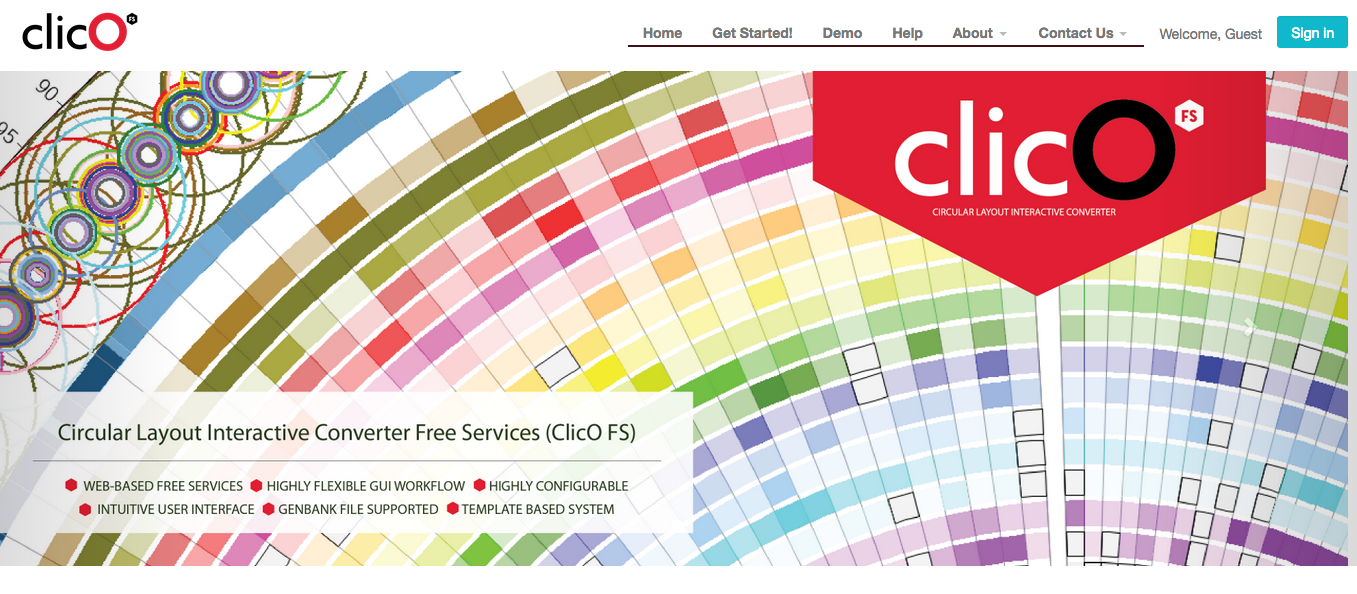
\includegraphics[scale=0.34]{figures/clico.png}}
  %\caption{ClicO, a free online tool for making circos plots}
  \label{fig:clico}
\end{figure}

\1 Click `Get Started!'
\1 Select `Blank Template'
\1 Click `Go'
\1 Enter in the details requested (Name of Project -$>$ Captcha -$>$ click `Start')

\begin{figure}[H]
  \centering
  \tcbox{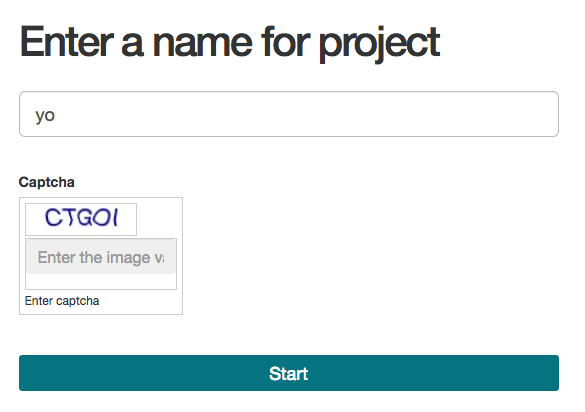
\includegraphics[scale=0.6]{figures/setup.png}}
  %\caption{Your project}
  \label{fig:setup}
\end{figure}

\end{outline}

\clearpage

\section*{Karyotypes}

\begin{outline}[enumerate]

\1 Click `$+$ Upload New'
\1 Add a name under `Description' and upload \textbf{karyotype.txt}
\1 Leave the default colour as is (we're overriding it anyway)
\1 Click `Upload'

\begin{figure}[H]
  \centering
  \tcbox{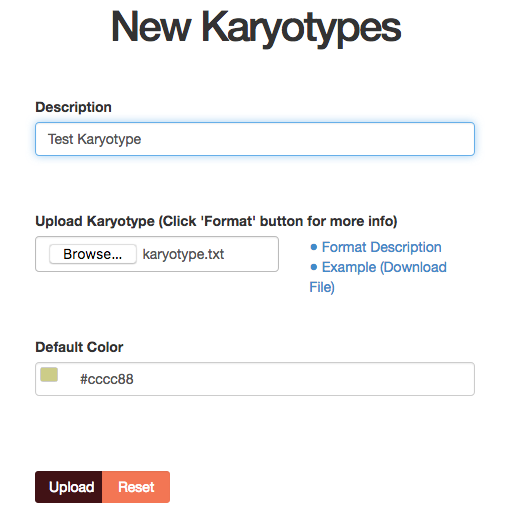
\includegraphics[scale=0.55]{figures/upload_karyotype.png}}
  %\caption{Upload your karyotype file}
  \label{fig:upload_karyotype}
\end{figure}

\1 Select the karyotype file you have just uploaded and proceed to the next step

\begin{figure}[H]
  \centering
  \tcbox{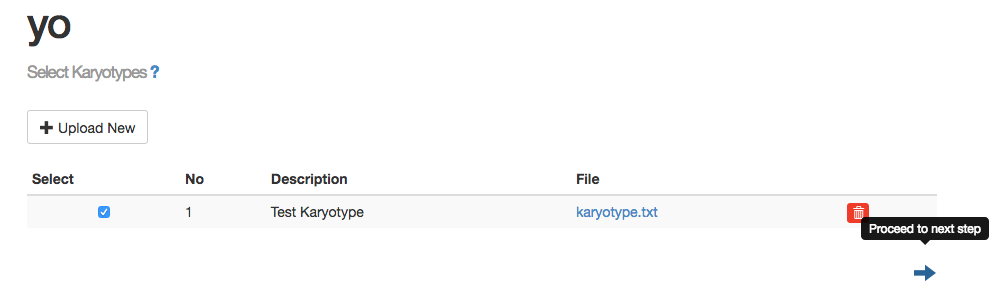
\includegraphics[scale=0.48]{figures/use_karyotype.png}}
  %\caption{Upload your karyotype file}
  \label{fig:use_karyotype}
\end{figure}

\clearpage

\1 Click `Preview' to have a look at the uploaded karyotype. 
This will be the backbone for your circos plot. 
You'll see that everything has automatically been filled in (e.g. each ``chr" or band, label, length and colour).

\begin{figure}[H]
  \centering
  \tcbox{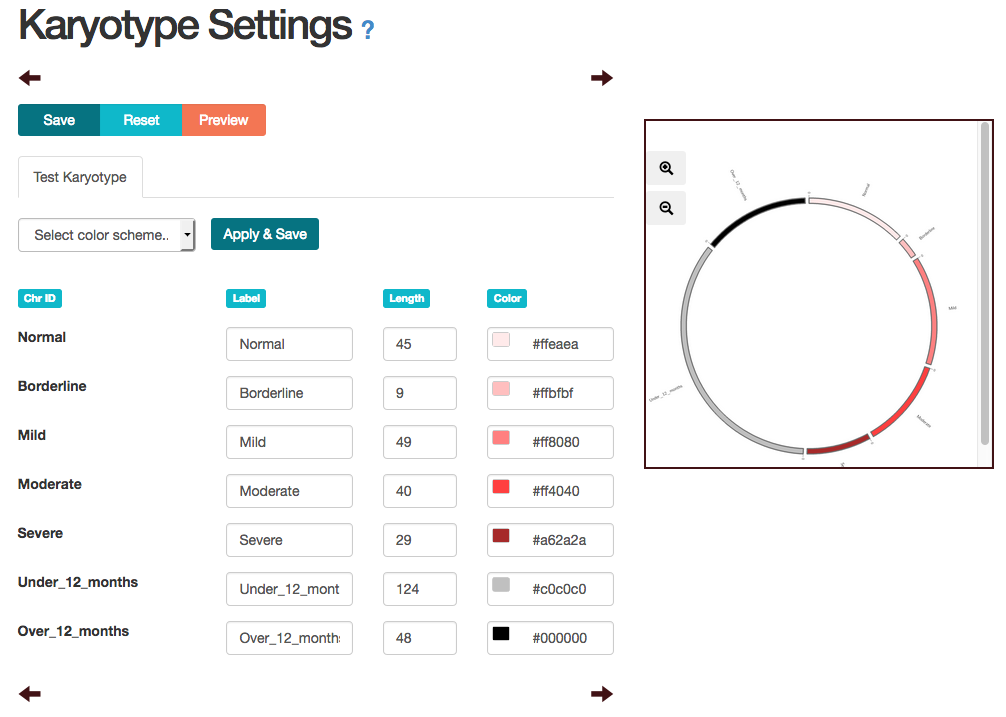
\includegraphics[scale=0.48]{figures/preview_karyotype.png}}
  %\caption{Upload your karyotype file}
  \label{fig:preview_karyotype}
\end{figure}
\end{outline}

\clearpage

\section*{Settings}

\begin{outline}[enumerate]

This section shows you how to tweak general settings like border colour, radius, thickness of your karyotype bands, label settings, tick settings, and so on. 
\textbf{It is very important to `Preview' and `Save' your changes as you go, or you will lose all changes.} At any time, you can go back or skip ahead to different settings options using the Settings menu at the top of the page.

\begin{figure}[H]
  \centering
  \tcbox{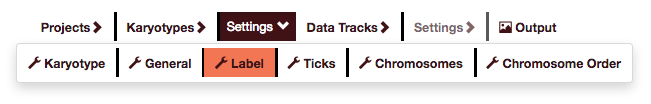
\includegraphics[scale=0.73]{figures/note_about_settings.png}}
  %\caption{Upload your karyotype file}
  \label{fig:note_about_settings}
\end{figure}

\clearpage

\1 First, we have general settings. Click `Preview' every time you make a change to see what it does. Once you're happy with the changes, click `Save' and go on.

I've changed the following:
	\2 \textbf{1 chromosome unit (u) represents 1: b (1 base)} 
		\3 This will add ticks at each ``base'', or in our case, for each individual. 
	\2 \textbf{Border thickness: 5} 
		\3 This reduces the thickness of the line around each band.
	\2 \textbf{Border color: \#120f0f} 
		\3 This changes the color of the border line to black.
	
\begin{figure}[H]
  \centering
  \tcbox{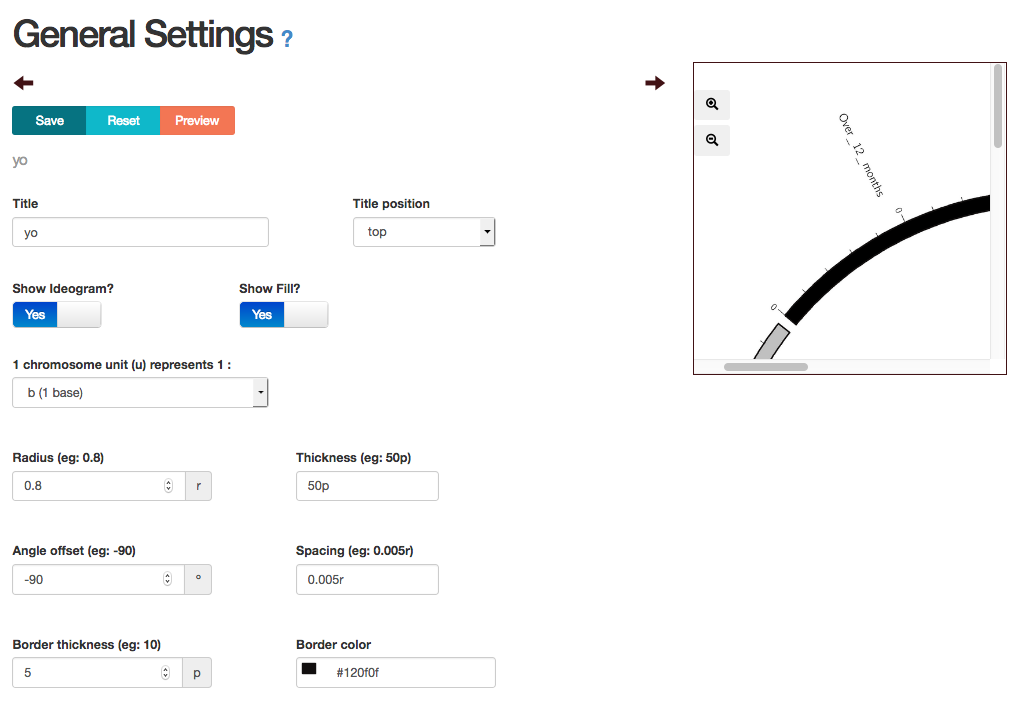
\includegraphics[scale=0.48]{figures/general_settings.png}}
  %\caption{Upload your karyotype file}
  \label{fig:general_settings}
\end{figure}

\clearpage

\1 Next, we have label settings. This controls your band labels. As before, make changes, `Preview' your changes, then `Save' once you're happy with them. 

I've changed:
	\2 \textbf{Parallel Label: Yes}

\begin{figure}[H]
  \centering
  \tcbox{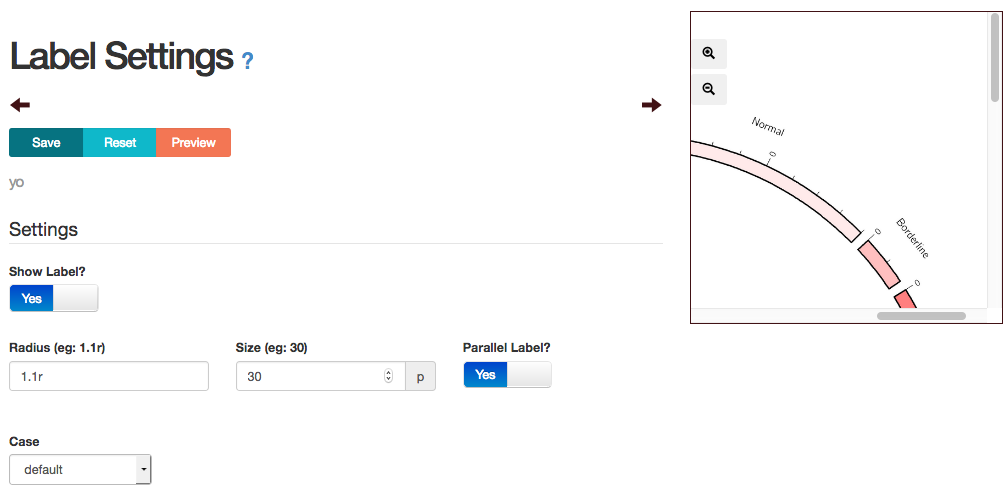
\includegraphics[scale=0.49]{figures/label_settings.png}}
  %\caption{Upload your karyotype file}
  \label{fig:label_settings}
\end{figure}

\clearpage

\1 For tick settings, I've changed:
	\2 \textbf{Label multiplier: 1e-0} 
		\3 This is the multiplier for the labels shown in the output. E.g. if we were drawing a genome and had position 20,000,000, we could set the multiplier to 1e-6 and then the label would be shown as 20. While this function is useful for genomes, we don't need it in this case. Setting it to 1e-0 will make each label appear as the real number.
	\2 \textbf{Major Ticks Label spacing: 5u}
		\3 Add a major tick at every 5 individuals.
	\2 \textbf{Minor Ticks Label spacing: 1u}
		\3 Add a minor tick at every 1 individual.
	
\begin{figure}[H]
  \centering
  \tcbox{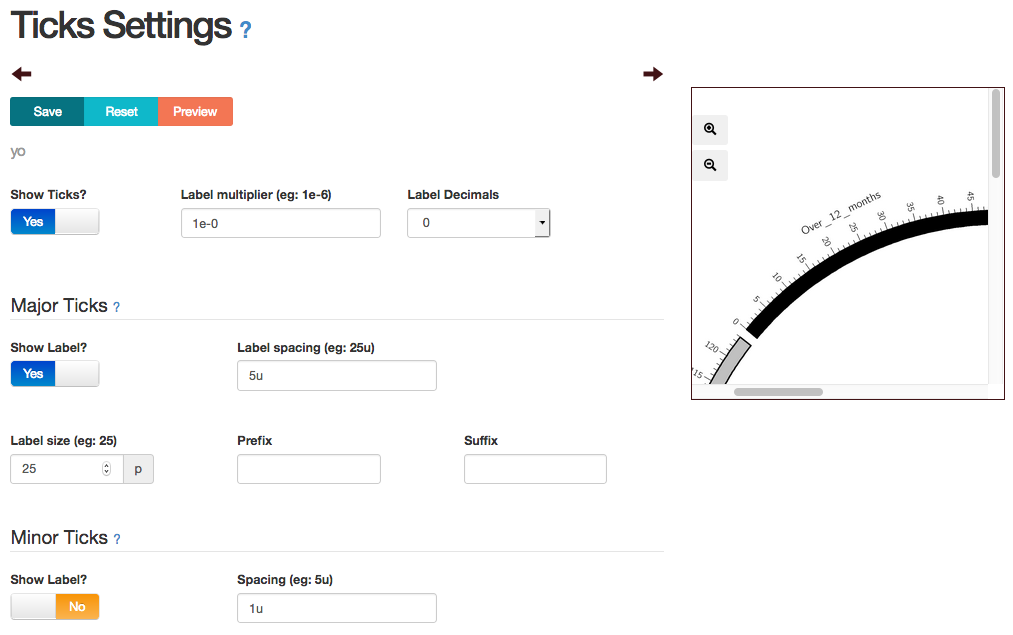
\includegraphics[scale=0.48]{figures/tick_settings.png}}
  %\caption{Upload your karyotype file}
  \label{fig:tick_settings}
\end{figure}	

\clearpage

\1 Finally, the chromosome settings are used to control which bands you want to appear and in what order. 
This can be useful if you want to have say Figure 1a as the whole genome, then Figure 1b as a close-up view of a particular chromosome. In our case, I left everything as default.

\begin{figure}[H]
  \centering
  \tcbox{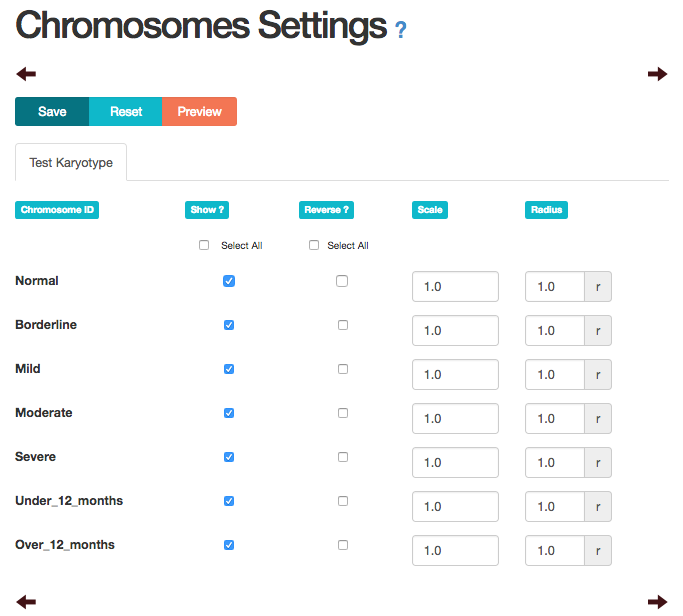
\includegraphics[scale=0.53]{figures/chromosome_settings.png}}
  %\caption{Upload your karyotype file}
  \label{fig:chromosome_settings}
\end{figure}	

\begin{figure}[H]
  \centering
  \tcbox{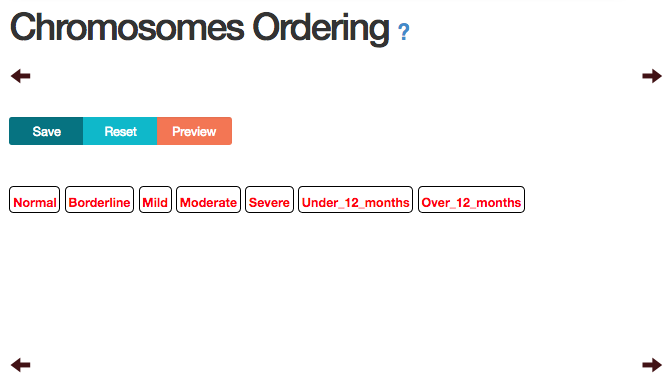
\includegraphics[scale=0.53]{figures/chromosome_order_settings.png}}
  %\caption{Upload your karyotype file}
  \label{fig:chromosome_order_settings}
\end{figure}	

\end{outline}

\clearpage

\section*{Data Tracks}

\begin{outline}[enumerate]

\1 Click `$+$ Upload New'
\1 Select File Type: Links (for this example, we'll be drawing connections between different bands)
\1 Add a description of your dataset (preferably something meaningful to you)
\1 Add the \textbf{data.txt} file
\1 Click `Upload'

\begin{figure}[H]
  \centering
  \tcbox{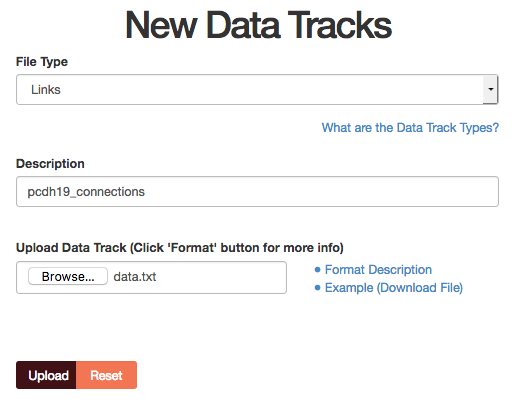
\includegraphics[scale=0.6]{figures/upload_data.png}}
  %\caption{Upload your karyotype file}
  \label{fig:upload_data}
\end{figure}

\1 Select (i.e. tick) your data set and continue.

\begin{figure}[H]
  \centering
  \tcbox{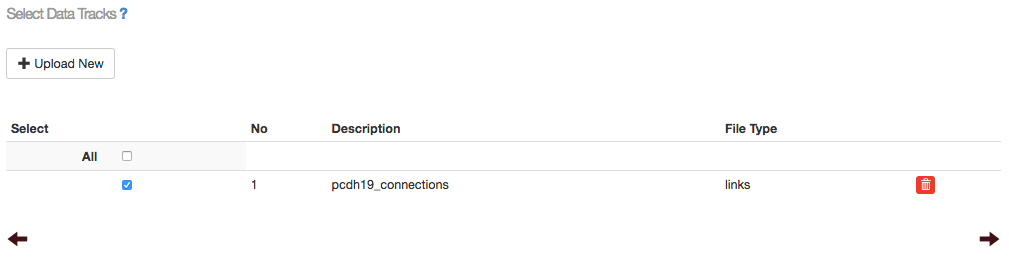
\includegraphics[scale=0.48]{figures/select_data.png}}
  %\caption{Upload your karyotype file}
  \label{fig:select_data}
\end{figure}

\clearpage

\1 There's only one page of data track settings. I like to specify everything in the \textbf{data.txt} file so that I don't need to change these settings manually. Note that anything you put in \textbf{data.txt} will override these manual settings. Click `Preview' to check that everything looks as expected.

\begin{figure}[H]
  \centering
  \tcbox{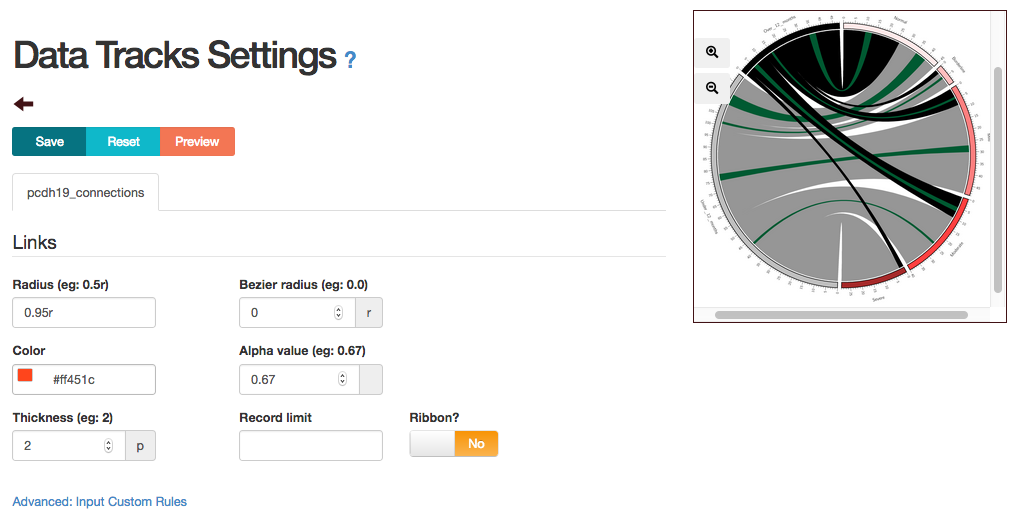
\includegraphics[scale=0.48]{figures/data_track_settings.png}}
  %\caption{Upload your karyotype file}
  \label{fig:data_track_settings}
\end{figure}

\end{outline}

\clearpage

\section*{Output}

To see your finished masterpiece, click `Output'.

\begin{figure}[H]
  \centering
  \tcbox{
\includegraphics[scale=0.62]{figures/output.png}}
  %\caption{Upload your karyotype file}
  \label{fig:output}
\end{figure}

It may take a while to load - you're probably due for a tea break now anyway.

\begin{figure}[H]
  \centering
  \tcbox{
\includegraphics[scale=0.48]{figures/loading.png}}
  %\caption{Upload your karyotype file}
  \label{fig:loading}
\end{figure}

\clearpage

{\Large And voil�!}

\begin{figure}[H]
  \centering
  \tcbox{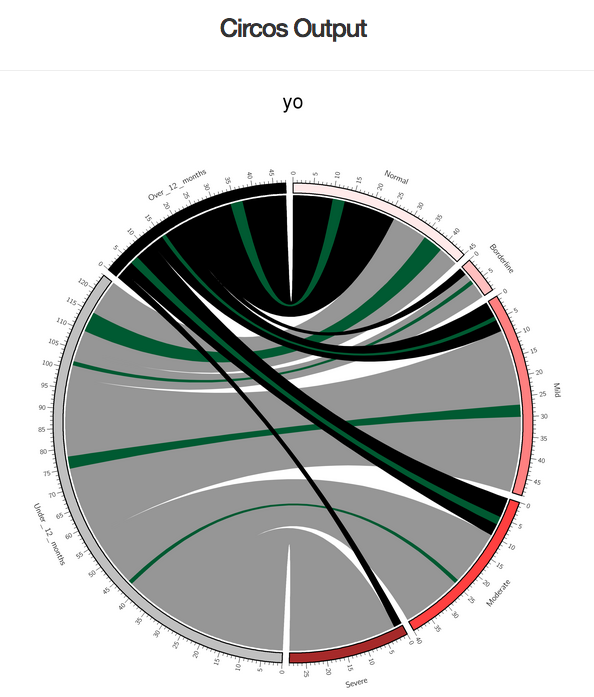
\includegraphics[scale=0.8]{figures/circos.png}}
  %\caption{Upload your karyotype file}
  \label{fig:circos}
\end{figure}

\clearpage

The two buttons in the top right let you download your output figure as a PNG or SVG file. 

\begin{figure}[H]
  \centering
  \tcbox{
\includegraphics[scale=0.8]{figures/download_images.png}}
  %\caption{Upload your karyotype file}
  \label{fig:download_images}
\end{figure}

And at the very bottom, you can also download the whole package of circos configuration files, if you want to make further changes directly using the command line circos package.

\begin{figure}[H]
  \centering
  \tcbox{
\includegraphics[scale=0.8]{figures/download_all.png}}
  %\caption{Upload your karyotype file}
  \label{fig:download_all}
\end{figure}

And there you go! Try it out and let me know how you go. I'll upload more templates soon...

	
} % this is the end brace for {\setlength{\parindent}{0cm}
\end{document}